\chapter{Low-fidelity prototyp}

\todo[inline, color=blue!30]{UPDATE: Postupně přidávám další kapitoly. Není dokončené, zatím v procesu.}

\todo[inline, color=blue!30]{Do téhle kapitoly by se ještě mělo vejít porovnání různých nástrojů a proč jsme se tak rozhodli.}

Po storyboardech, které nám ukázali možné sekvence akcí, vytvoříme prototyp aplikace, se kterým budou interagovat uživatelé. V rámci ročníkového projektu vytvoříme jen low-fidelity prototyp. Tedy se budeme zabývat vytvořením rané verze aplikace, která nebude věrnou kopií aplikace výsledné. V této fázi, chceme hlavně rychle vytvořit prototyp, na kterém můžeme vyhodnocovat nápady a zároveň ho můžeme otestovat na uživatelích spadajících do jednotlivých uživatelských skupin, které jsme si definovali.

\section{Paper prototyping}

Pro navrhování a testování uživatelského rozhraní, ve verzi low-fidelity, jsme si vybrali hojně využívanou metodu prototypování na papír (paper prototyping). Celý proces od vytvoření prototypu až po uživatelské testování popisuje detailně kniha Paper prototyping od Carolyn Snyder \cite{Paper_Prototyping}.

Začneme vytvořením papírových komponent aplikace (oken, menu, stránek, dialogových boxů, dat, pop-up zpráv). 
Po vytvoření prototypu provedeme usability otestování.
V takovém testování provádí uživatel, v jednom sezení, realistické úkoly na papírovém prototypu. Nejedná se o studii, kdy jsou prováděny série testů použitelnosti během několika dní. Uživatelé jsou vybraní podle uživatelských skupin, které jsme si definovali na začátku.

Prototyp bude ovládaný osobou, která reprezentuje konání počítače, ale nevysvětluje, jak má rozhraní fungovat. Další zkušený člověk funguje jako zapisující pozorovatel. Pozoruje chování uživatele, zapisuje co uživatel dělá a co říká. Tímto způsobem provedeme velmi rychle iterativní testování na několika uživatelích. V průběhu můžeme aplikaci vylepšovat a všímat si opakujících se vzorů. Každé sezení s uživatelem končí vyplněním dotazníku spokojenosti s aplikací.

\section{Low-fidelity návrh}

Low-fidelity návrh vytvoříme v nezávislosti na existujících aplikacích. V tomto momentě je dobré si ujasnit, na jakém zařízení budeme aplikaci používat. Tak nějak implicitně jsme od začátku předpokládali, že půjde o počítačové rozhraní. Mobilní aplikace se k němu nepřidá, alespoň ne ve verzi s možností úprav. Stejně tak aplikace pro tablety. Tahle zařízení jsou užší a menší. Mají tak méně prostoru pro obsah, navigaci a interakci. Použití modelovacích a složitějších funkčností by tak bylo často složité až nemožné.

Zaměřili jsme se na to, jestli jsou komponenty dostupné, jestli nic nemate uživatele, když má na něco kliknout...

Když se má uživatel někam dostat, tak aby ho nerozptylovaly komponenty a věděl na co chce kliknout

jako inspirace nám posloužili nástroje... (všechny nástroje na webu, protože navrhujeme aplikaci na webu -> uvést tuhle informaci někde nahoře)

nesnažíme se z toho dělat vyloženě závěry, jenom se snažíme poukázat na podobnosti s návrhem person

Ukázat několik aplikací a porovnat, proč jsme se rozhodli tak a tak to udělat (jedna z nich https://app.sqldbm.com/PostgreSQL/DatabaseExplorer/Draft/). F-Pattern, kam se dostanu po kolika kliknutích, F-Pattern se nehodí pro telefony, je dobré F-Pattern použít jako základ, ale vyloženě se tím neřídit (dnes spíš tíhne k rozmanitosti), The F-Pattern is mirrored in right-to-left languages, such as Arabic, aplikace psaná anglicky -> jsme zvyklí číst zleva doprava

\begin{figure}[htb]
    \centering
    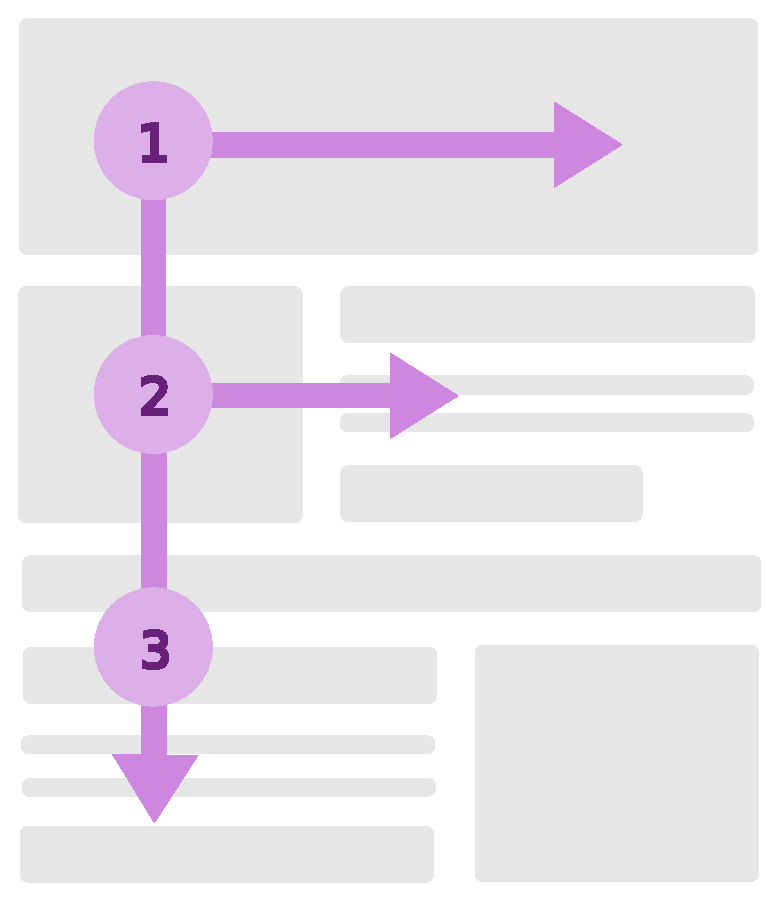
\includegraphics[height=70mm]{../img/F-Pattern}
    \caption{F-Pattern layout.}
    \label{obr03:fpattern}
  \end{figure}

Subsekce na:
- existující nástroje, kterýma jsme se inspirovali
- konkrétní návrh -> popsání hlavní obrazovky, zaměření se na plovoucí komponenty

\section{Uživatelské testování}

\todo{Do téhle podkapitoly dát obrázek z průběhu uživatelského testování}

Proč je dobré takový návrh vůbec testovat na uživatelích? (krom toho, že ho můžeme rychle měnit) str. 58 z \cite{Paper_Prototyping} No nitpicky (hnidopišský) feedback. Pokud se chceme vyhnout hnidopišské zpětné vazbě, může nám pomoct low-fidelity návrh. Komponenty nejsou jasně dané, uživatel se spíš zaměří na koncepty a funkčnost. Je totiž očividné, že jsme ještě nespecifikovali vzhled. Zároveň to povzbuzuje uživatele, aby nebyl pasivní, ale sám kreativně přemýšlel nad koncepty. Dokonce není neobvyklé měnit vzhled s uživatelem přímo při testování. Tím, že nedokončený návrh povzbuzuje ke kreativitě, se zabývali výzkumníci v článku \cite{Schumann_1996_AEN}.

Techniky pro pozorování uživatelů. Chceme se připravit, pro maximalizaci užitečnosti dat z otestování. Kroky pro pozorování uživatelů, tak abychom na konci věděli, kde mají uživatelé problém aplikaci používat. 
Připravit si úkoly, které budou uživatelé dělat. Mělo by se jednat o reálné úkoly, které budou uživatelé v aplikaci nejběžněji dělat. 
Dál najít uživatele co sedí na persony. Dávat si pozor, aby neznali aplikaci nebo naše názory na ni.
Pro testování vybrat místo, které je tiché a bez zbytečných vnějších vyrušování.
Popsat uživateli o co se jedná, že jsou zapojeni do raných fází návrhu. Zdůraznit, že testujeme aplikaci, ne uživatele.
Poprosit uživatele aby přemýšleli nahlas, aby říkali to co jim přijde na mysl, v průběhu plnění úkolů. Díky tomu prozkoumáme jejich očekávání od produktu, taky jejich úmysly a jejich strategie řešení problémů.
Upozornit, že nebudeme uživateli pomáhat při plnění úkolů. Je to nejlepší způsob jak zjistit jak uživatelé reálně interagují s aplikací. 
Po testování zodpovědět zbývající otázky od uživatele. Lze diskutovat, nějaké zajímavé chování, které uživatel měl při testování. Zeptat se na celkový dojem z aplikace. Tohle je popsané v knize \cite{Brenda_1990_art} (kapitola Some Techniques for Observing Users)

V dotazníku (a obecně) jenom otevřené otázky (abychom nikoho nenaváděli).


